\title{Concurrency and Parallel Programming \\ Assignment 2}
\author{David van Erkelens and Jelte Fennema \\ Department of Computer Science
    \\ University of Amsterdam} \date{\today}
\documentclass[12pt]{article}
\usepackage{graphicx}
\usepackage{color}
\begin{document}
\maketitle
\section{Wave}
\subsection{Comparison with self defined threads}
Both graphs show that for some unknown reason the largest problem size performs worse than a problem size smaller. The problemsize $10^6$ performs best in both cases and the speedup is about the same except when using 8 threads.\\
OpenMP gets a good speedup when using $10^4$, this is definitly not the case when using self defined threads.\\
When looking at all problemsizes, OpenMP gets the best speedup for small problemsizes and self defined threads get the best speedup out of the larger problemsizes.
\subsection{Chunksize and scheduling technique}
This test was done with an i\_max of $10^6$, a t\_max of $20000$ and using eight threads.
\subsubsection{Static}
When using a small chunk sizes, the static scheduler spends quite a bit of its time deviding the chunks over the threads. When using chunck sizes betweent 2500 to 250000 it performs the best. After the 250000 the performance goes down again since the load can't be balanced as well anymore.
\subsubsection{Dynamic}
When using really tiny chunk sizes the performance of the dynamic scheduler is utterly terrible. With a chunk size of one this scheduler timed out, which means it went over the 900 seconds and with a chunk size of 5 it still spends most of its time deviding the chunks. After that it stagnates a bit, but is still slower than the static scheduler with most of the chunk sizes. After the 250000 the performance of this scheduler goes down as well.

\subsubsection{Guided}
The performance of this scheduler doesn't really get influenced by the chunk size. Only the logical slowdown when the chunk size gets really large can be noticed. 

\subsubsection{Conclusion}
The static scheduler has the best performance when the chunk size is chosen somewhere between about a $1/400$ and a $1/4$ of the iteration maximum. The dynamic scheduler performce mediocre when comparing it to both other schedulers, although it can perform better than the guided scheduler when the chunk size is chosen just right. The guided scheduler performs better than the static with small chunk sizes, so when you don't care about specifying a good chunk size it is a good choice.

\clearpage
\subsection{Graphs}
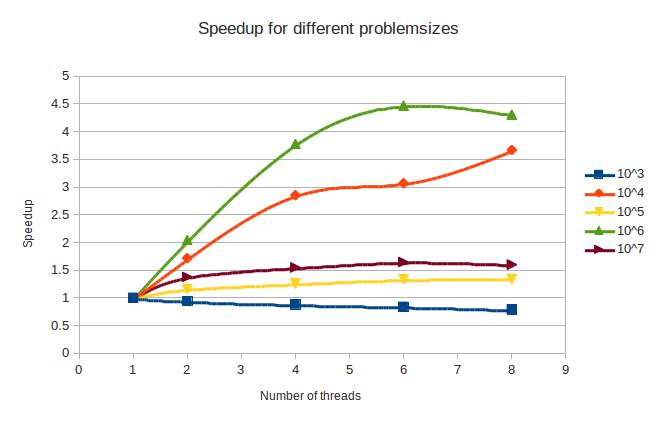
\includegraphics[width=\textwidth]{threads.jpg}
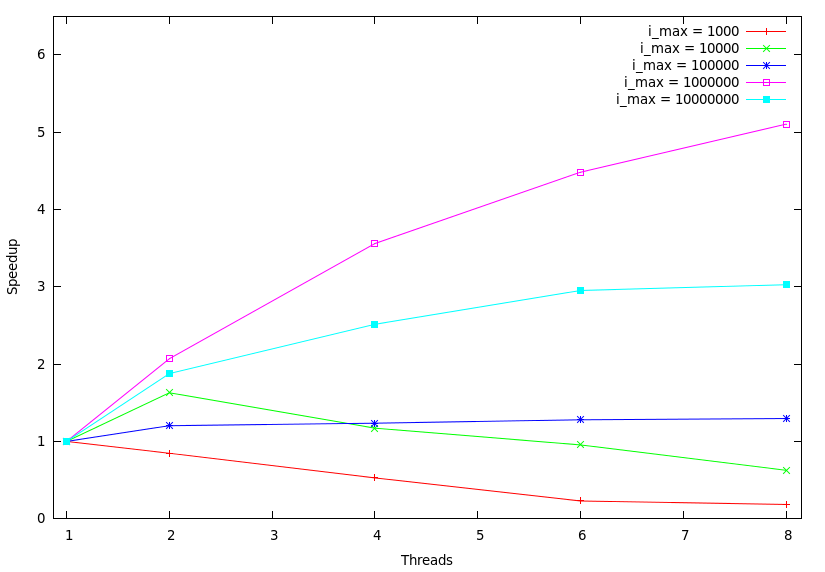
\includegraphics[width=\textwidth]{speedupgraph.png}
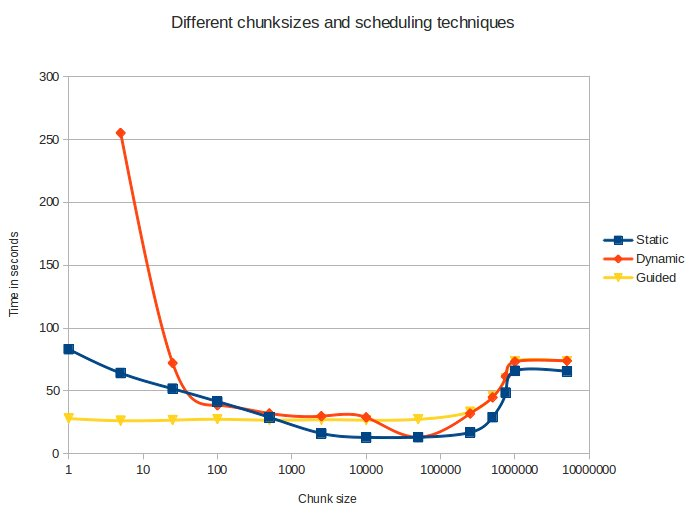
\includegraphics[width=\textwidth]{chunks.jpg}
\section{Mandelbrot}

\end {document}
